\section{Evaluation}
\label{sec:eval}

\subsection{Experimental Setup}

\subsubsection{Hardware}

We ran our tests on a mid-2012 MacBook Pro with a 2.6 GHz Core i7 processor,
8GB RAM, and an NVIDIA GeForce GT 650M graphics card with 1GB memory.


\subsubsection{Router Framework}

We implemented a software router framework capable of running in one of two
modes: CPU-only or CPU/GPU. We use the router in CPU-only mode to gather a
baseline against which we can compare the performance of CPU/GPU mode. In
either mode, the framework handles gathering batches of packets, passing them
to a ``pluggable'' packet processing function, and forwarding them based on the
results of processing. 

We implemented three processing functions: one that does longest prefix match,
one that does firewall rule matching, and one that does both. For each we
implemented CPU version and a GPU version (the GPU version is a CUDA kernel
function).

\subsubsection{Packet Generation}
We use the Click Modular Router \cite{kohler2000click} to generate packets for our
software router framework to process. We modify the standard packet generation
functions in click to output UDP packets with random source and destination
addresses as well as random source and destination ports. We have click generate
these randomly addressed packets as fast as it can and have it send the packets
up to our software routing framework via a standard Berkeley socket between both
locally hosted applications.

Note that this ``full-on'' kind of workload is essential to test the maximum
throughput of our router framework, but does not necessarily model a particular
kind of real-world workload. However, in the case of our system, we wish to
measure the feasibility of processing packets in software at the same speed as
specially-designed hardware ASICs. Thus our evaluation focuses on comparisons
of maximum throughput.

\subsubsection{Packet Processing}
\label{sec:eval-proc}

\noindent \textbf{Longest Prefix Match.} First of all, since CUDA provides
limited support for dynamic data structures such as a trie, we adapted the
algorithm to run on the GPU. In particular, in the initial setup of the trie,
we serialize the data structure into an array, so that it can be easily
transferred on the GPU's memory.

In order to work with a realistic dataset, we initialized the FIB with the
prefixes in the Internet belonging to actual Autonomous Systems. The list has
been retrieved from CAIDA \cite{routeviews}, which periodically stores a
simplified version of its RouteViews Collectors' BGP tables. Overall, the size
of the trie turns out to be a few tens of megabytes large. Once built, the
serialized trie is transferred to the GPU to be used during lookup.


\noindent \textbf{Firewall Rule Matching.} To evaluate the performance of our
router's firewall rule matching function, we generate a set of random firewall
rules. The 5-tuple values for our random rules are chosen according to the
distributions in \cite{Rovniagin}. For example, we use the probabilities in
Table~\ref{tab:proto-dist}, taken from \cite{Rovniagin}, to pick a new random
rule's protocol. Similar statistics were used to pick source/destination
address/port.

\begin{table}[htbp]
   \centering
   \begin{tabular}{ l l } 
      \toprule
      \textbf{Protocol}  & \textbf{Prevelance in Rules} \\
      \midrule
	  TCP & 75\% \\
      UDP & 14\% \\
	  ICMP & 4\% \\
	  * & 6\% \\
	  Other & 1\% \\
      \bottomrule
   \end{tabular}
   \caption{Protocol distribution in firewall rules}
   \label{tab:proto-dist}
\end{table}

\subsection{Evaluation Metrics}
\label{sec:metrics}

We use three different metrics to evaluate our router's performance. The results
in \S\ref{sec:results} present these values averaged over 30 seconds of router
operation.

\medskip \noindent \textbf{Bandwidth.} No router performance evaluation would
be complete without considering bandwidth, and so we measure the number of 64
byte packets forwarded by our router per second, from which we calculate
bandwidth in gigabits per second. For comparison, the norm for core routers is
about 40 Gbps with high-end routers currently maxing out around 100 Gbps.

\medskip \noindent \textbf{Latency.} Bandwidth only tells part of the story,
however; the delay a single packet experiences at a router is important as well
(for some applications, it is more important than bandwidth). Since some
optimizations aimed at increasing our router's bandwidth increase latency as
well (such as increasing batch sizes), measuring latency is important.

We measure both the minimum and maximum latencies of our router. The maximum
latency is the time from the arrivial of the first packet of a batch to the
time it is forwarded; the minimum latency is the same but for the last packet
of a batch.

\medskip \noindent \textbf{Processing Time.} We also consider a microbenchmark:
the time spent in the packet processing function itself (i.e., doing the longest
prefix match lookup or matching against firewall rules). This is largely a
sanity check; we expect to see the GPU perform much better here, though actual
performance (measured by bandwidth and latency) depends on many other factors
(like the time spent copying data to/from the GPU).


\subsection{Results}
\label{sec:results}

Our router went through four iterations, each one introducing optimizations
based on what we learned from the results of the last. We therefore present our
results in four stages, guiding the reader through our design process.

\subsubsection{Iteration One}

We began by na\"{i}vely implementing the design presented in
\S\ref{sec:system-design}; at this point, we made no optimizations --- the goal
was building a functioning GPU-based router.

Not surprisingly, it performed underwhelmingly. The GPU version of our router
achieved roughly 80\% of the bandwidth the CPU version did
(Figure~\ref{fig:iter1-bw}) and its (max and min) latencies were 1.3X longer
(Figure~\ref{fig:iter2-lat}). The processing time is not to blame; as expected,
the GPU performs the actual packet processing much faster than the CPU
(Figure~\ref{fig:iter1-proc} --- the GPU processing time is so small it hugs
the X axis). A quick examination of the time spent performing different
functions (Figure~\ref{fig:iter1-gpu-breakdown}) explains where the GPU router
is losing ground: although it spends less time processing, it has to copy
packets to the GPU for processing and copy the results back, tasks the CPU
version doesn't need to worry about (Figure~\ref{fig:iter1-cpu-breakdown}).

\begin{figure}
    \centering
    \subfigure[Bandwidth vs. Batch Size]{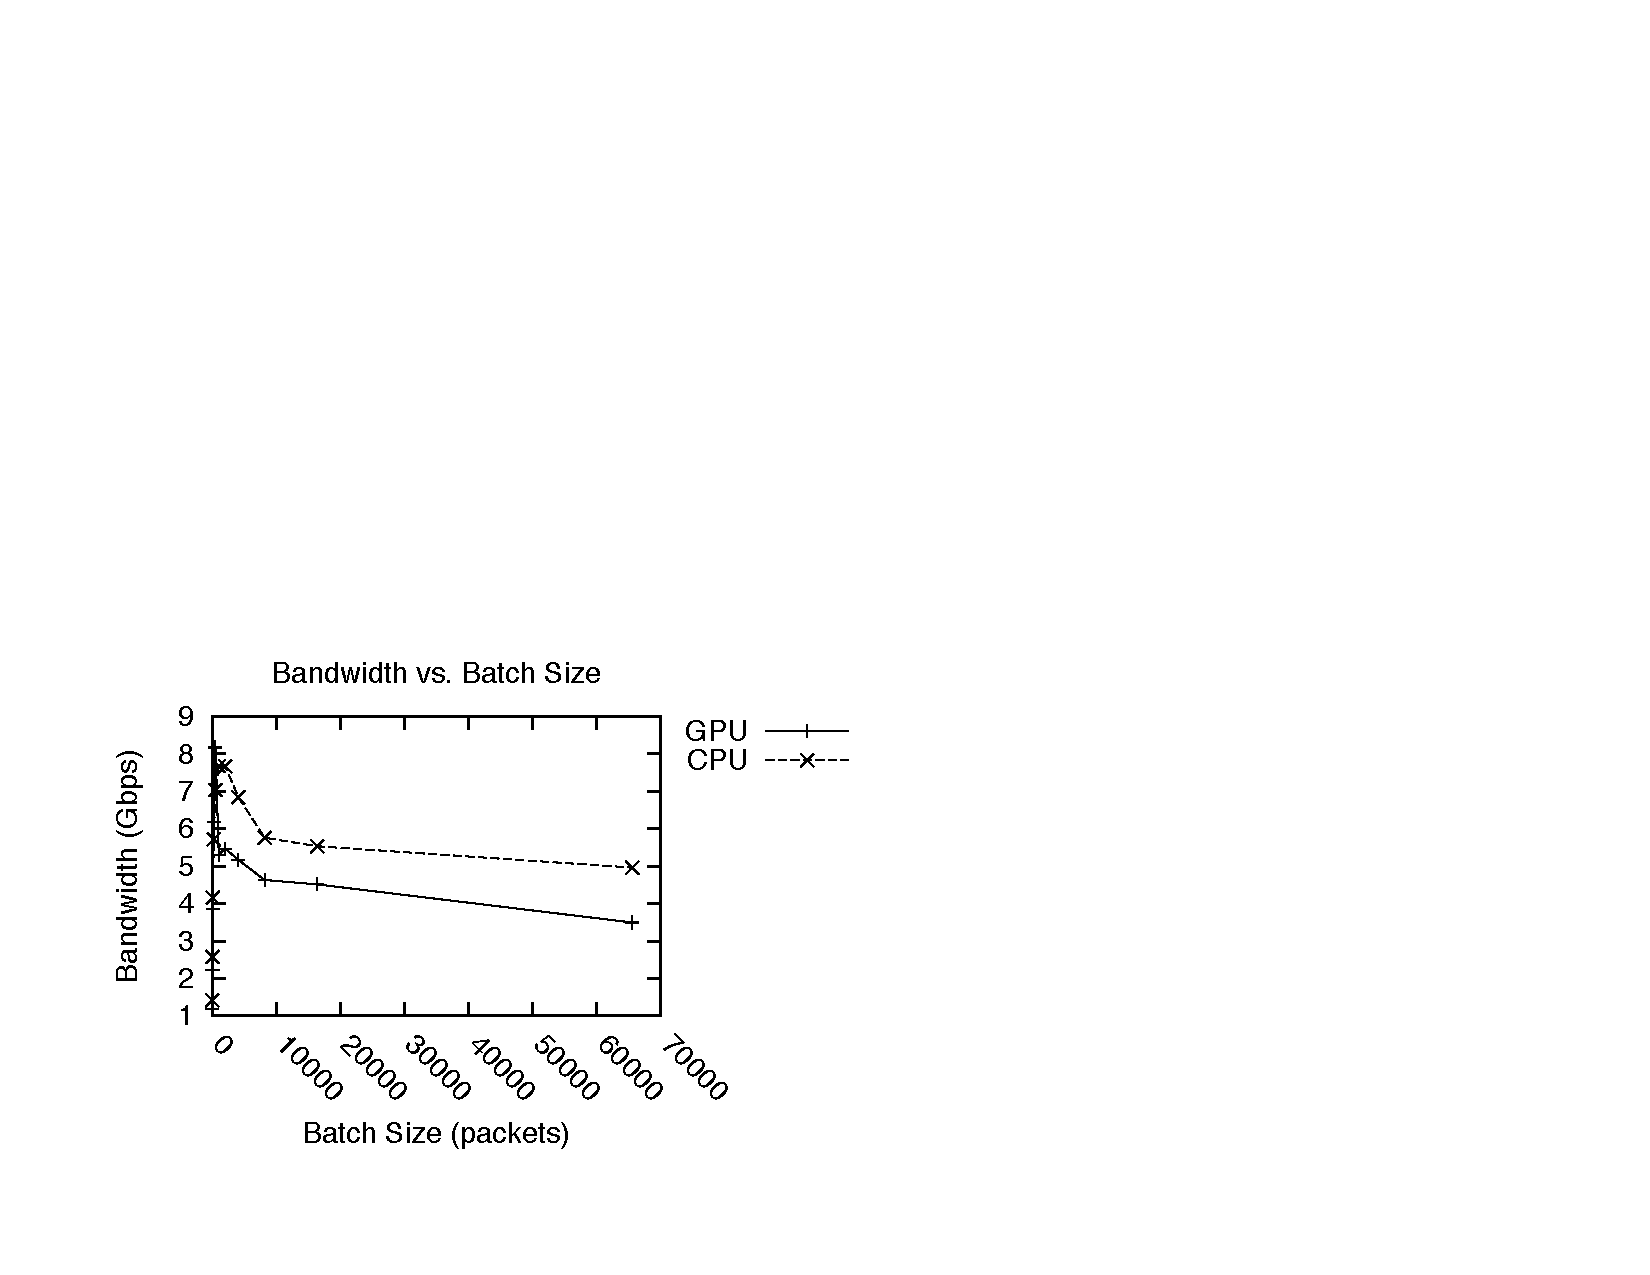
\includegraphics[height=3.5cm]{figs/batch_size_both_par_bw.pdf}\label{fig:iter1-bw}}
	\medskip

    \subfigure[Latency vs. Batch Size]{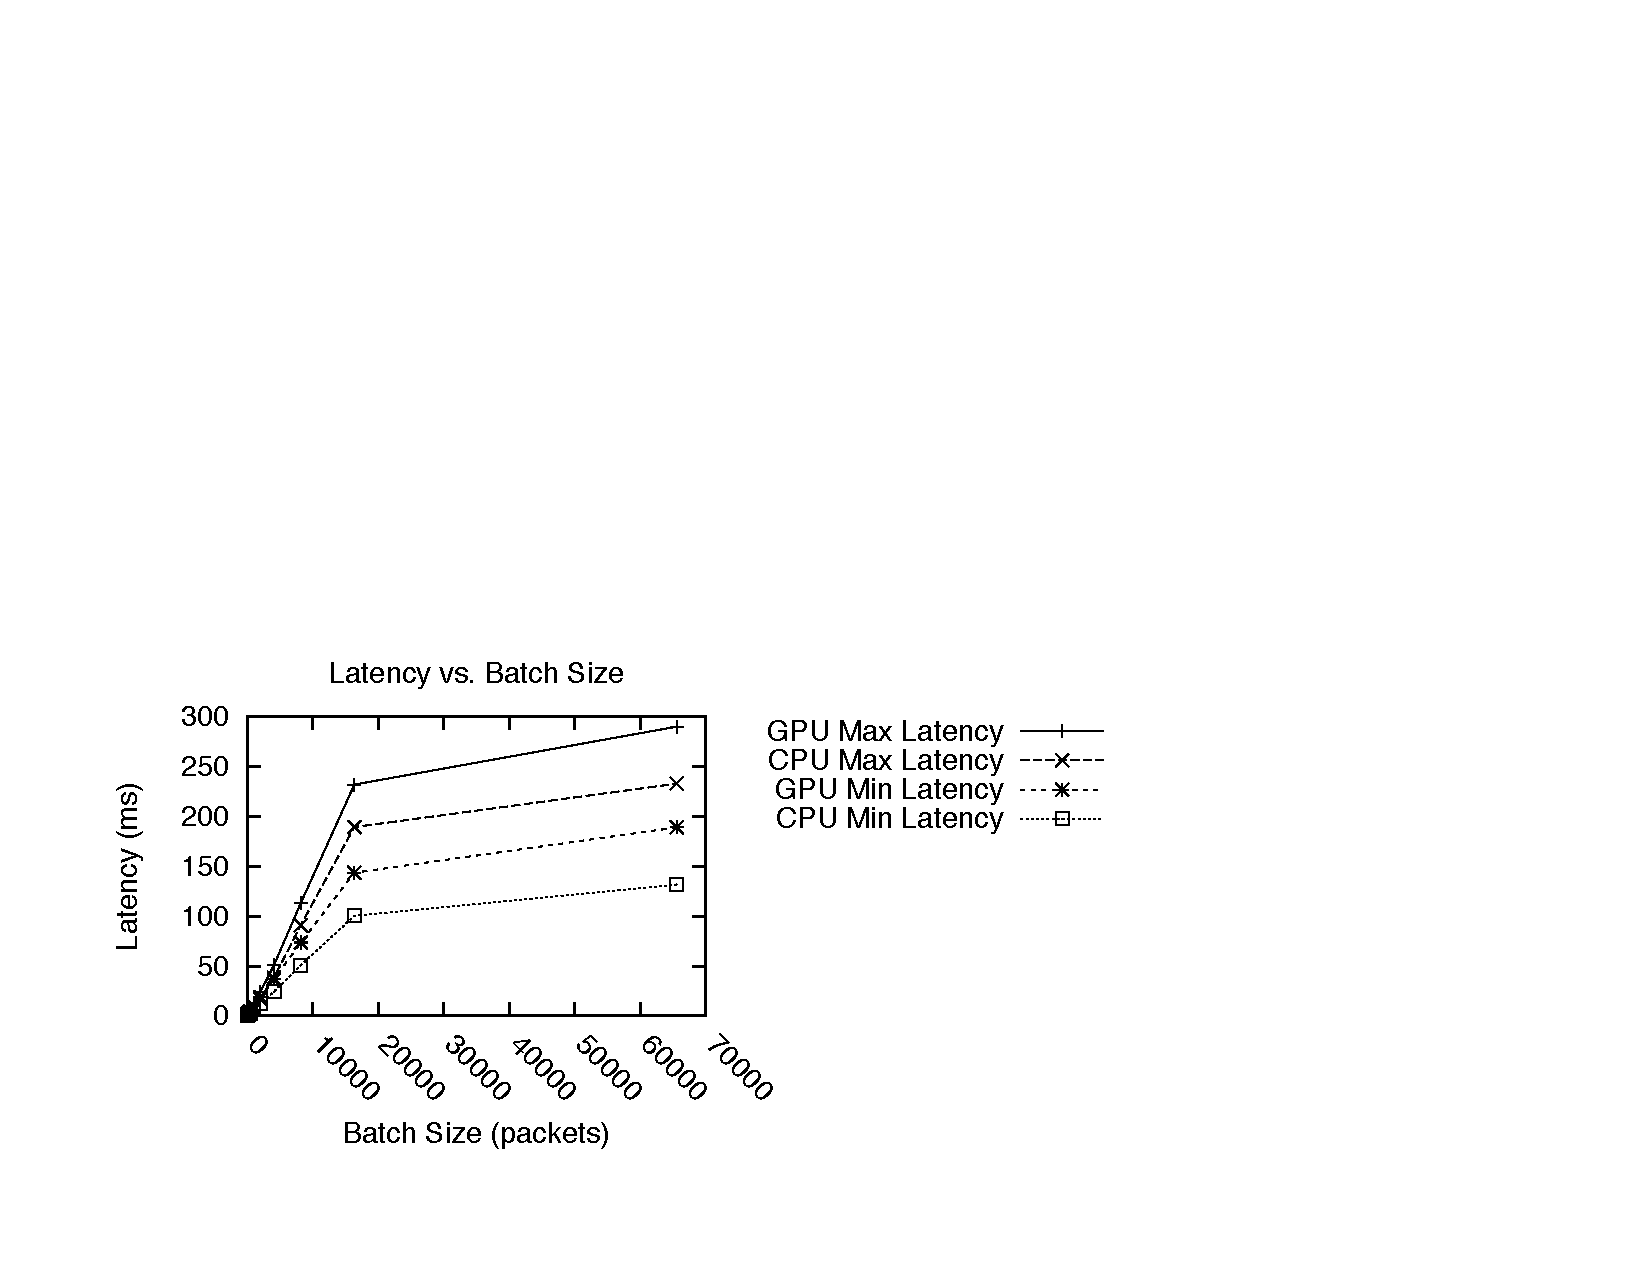
\includegraphics[height=3.5cm]{figs/batch_size_both_par_lat.pdf}\label{fig:iter1-lat}}

	\medskip
    
	\subfigure[Processing Time vs. Batch Size]{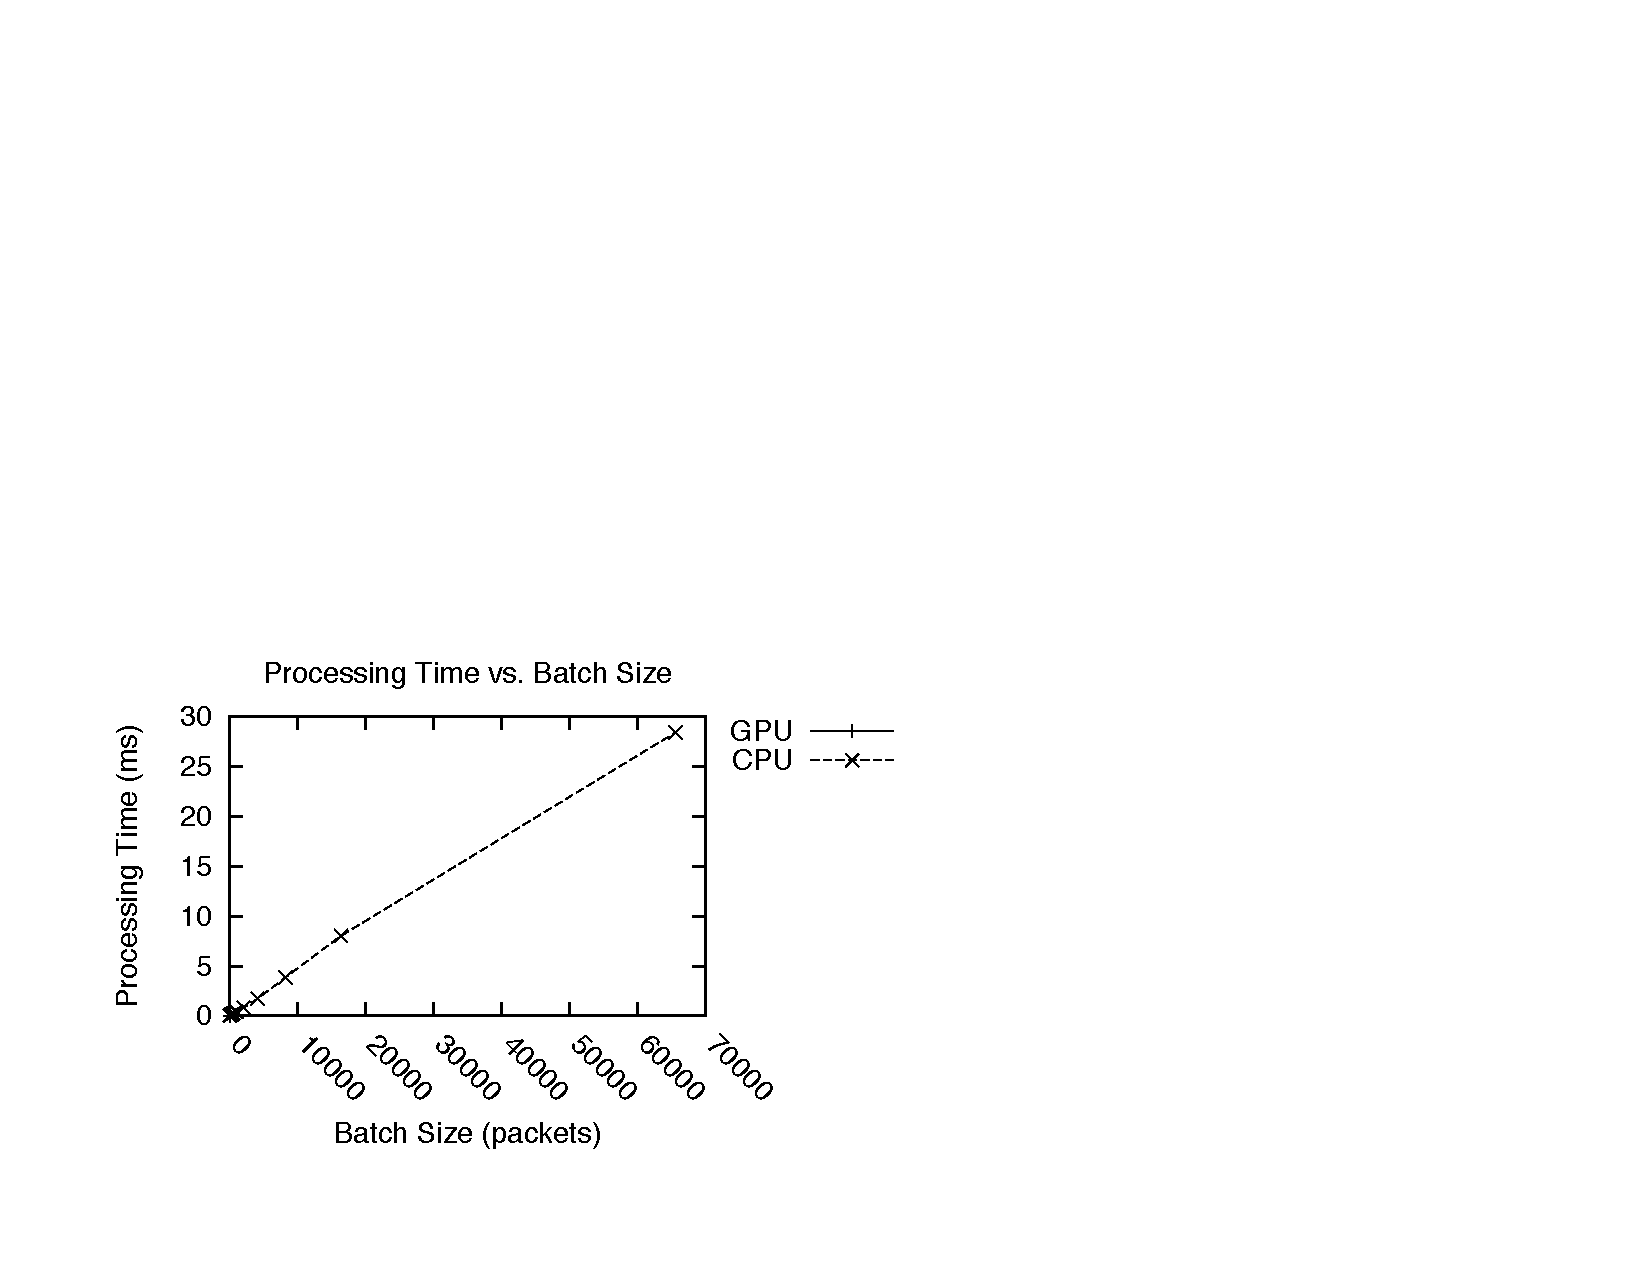
\includegraphics[height=3.5cm]{figs/batch_size_both_par_proc.pdf}\label{fig:iter1-proc}}
	\medskip
	
	\subfigure[Breakdown of Relative GPU Time]{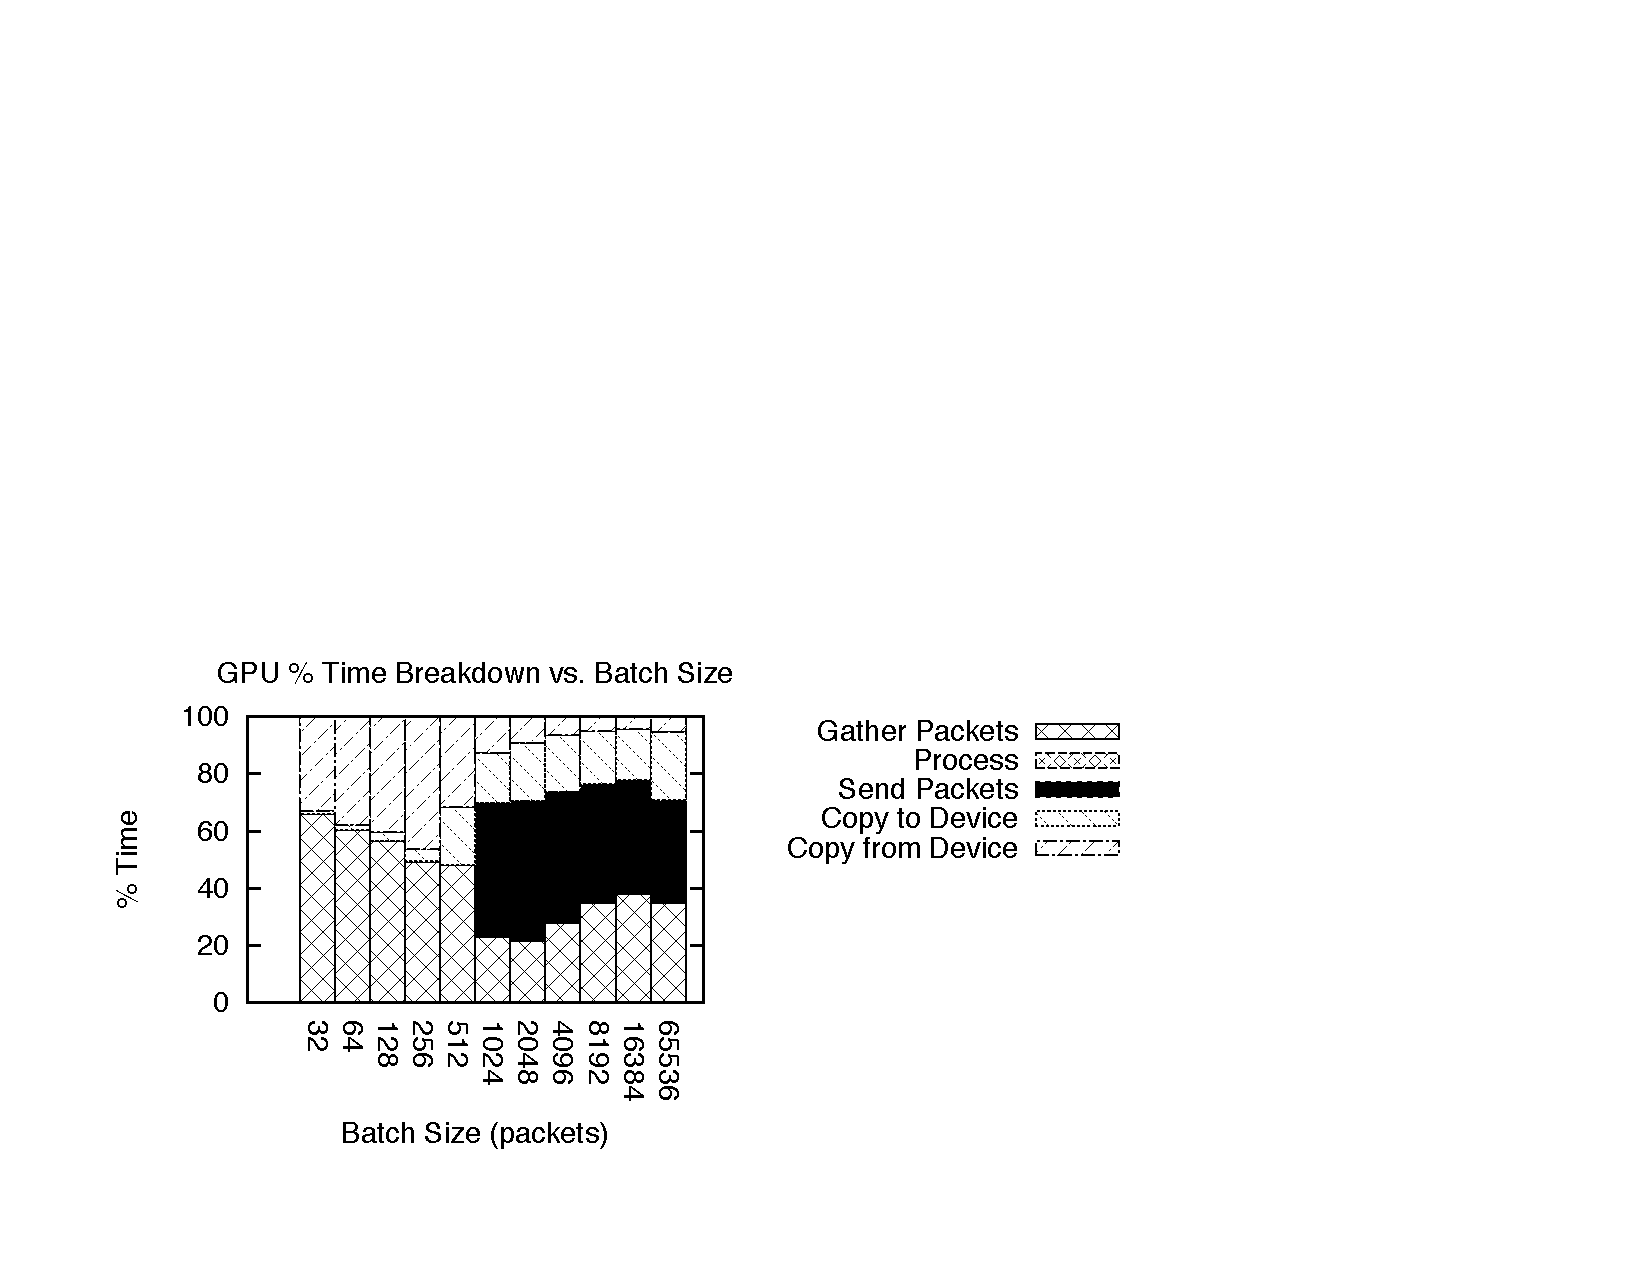
\includegraphics[height=3.5cm]{figs/batch_size_both_par_gpu_p.pdf}\label{fig:iter1-gpu-breakdown}}
	
	\medskip
	\subfigure[Breakdown of Relative CPU Time]{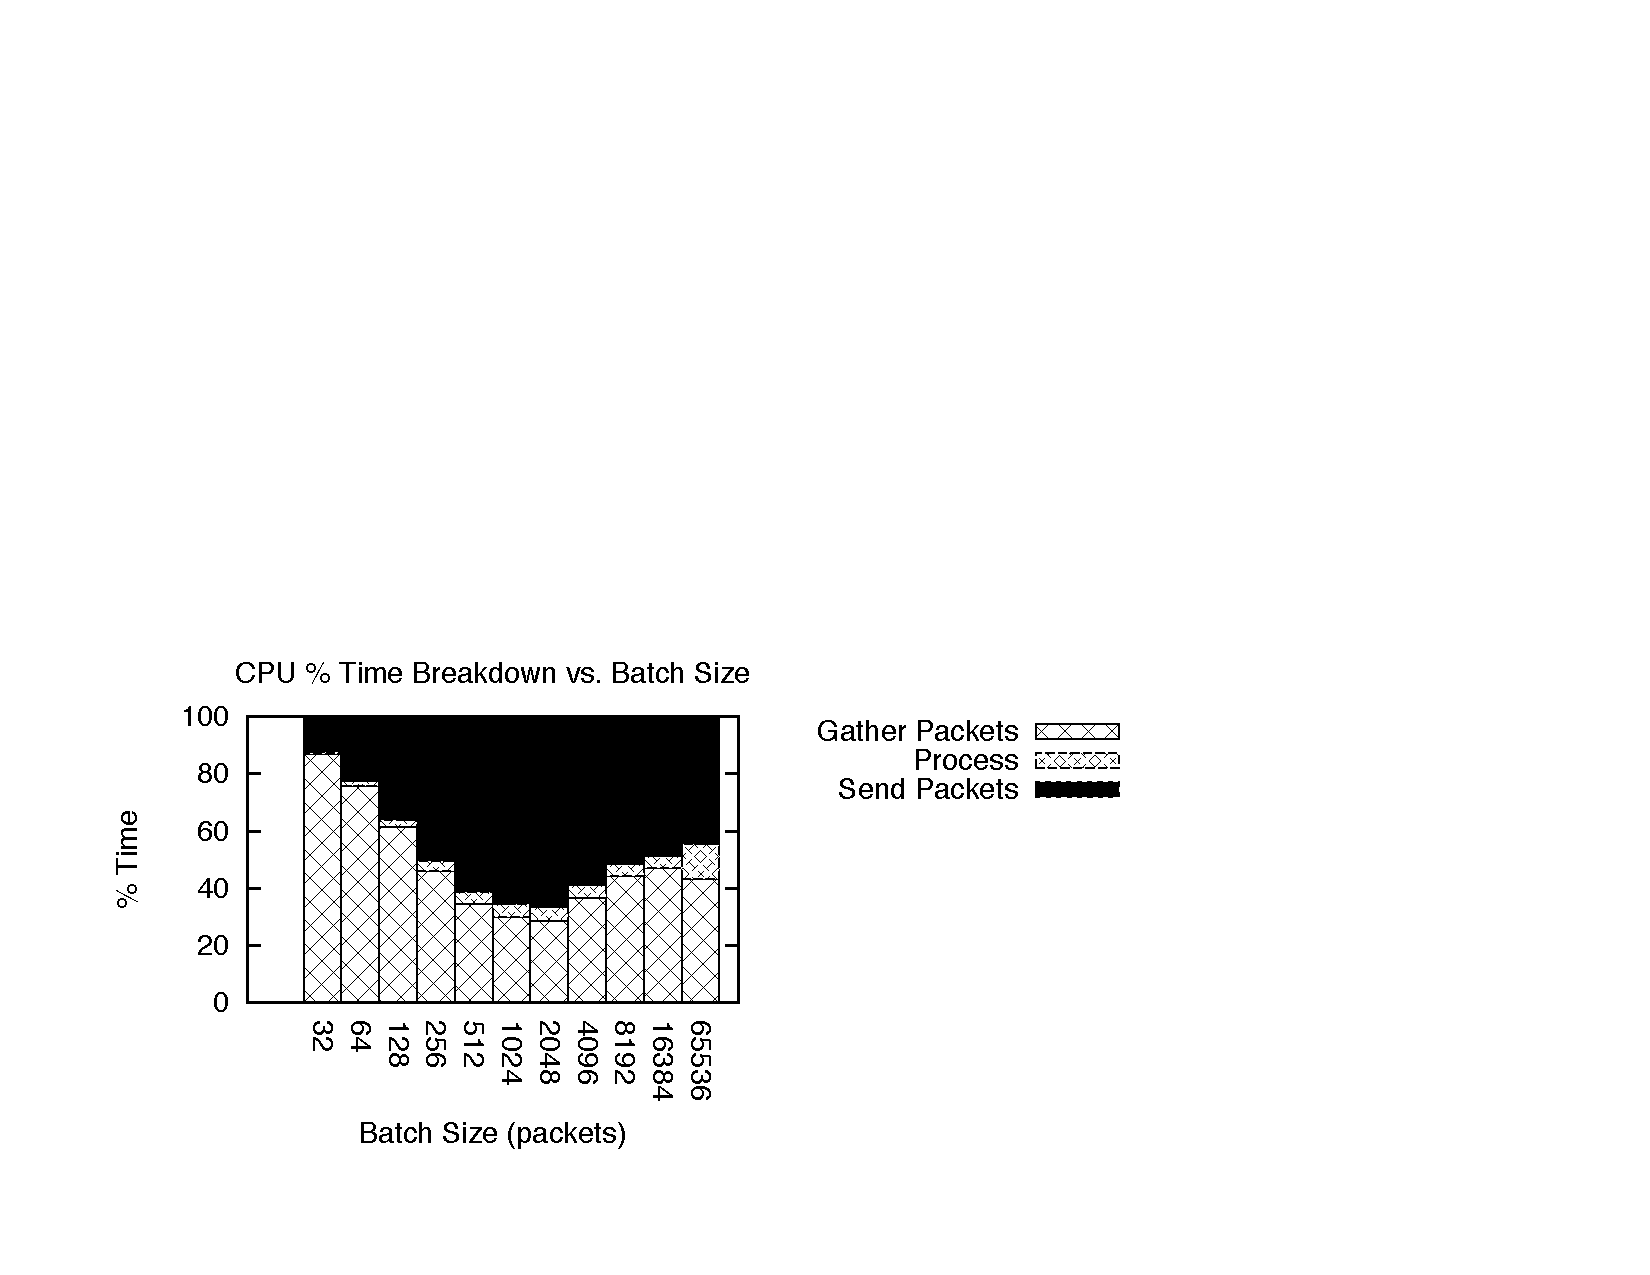
\includegraphics[height=3.5cm]{figs/batch_size_both_par_cpu_p.pdf}\label{fig:iter1-cpu-breakdown}}

    \caption{Iteration 1 Results}
	\label{fig:iter1}
\end{figure}


\subsubsection{Iteration Two}

Since both of our packet processing functions operate only on the data carried
by the packet header, we can reduce the time spent copying data to the GPU by
copying only the packet headers. Unfortunately, the results do not contain
unnecessary information, and cannot easily be condensed (this is not completely
true --- it is probably possible to compress the results, though we do not
explore this here).

Figure~\ref{fig:iter2} shows the performance of the second iteration of our
router. Reducing the number of bytes copied to the GPU has closed the gap
between the CPU-only and the CPU/GPU routers in terms of bandwidth and latency,
but the CPU/GPU router still doesn't perform any better. Even though we have
all but eliminated copy time to GPU, Figure~\ref{fig:iter2-gpu-breakdown}
suggests that we should try to cut down copy time from the GPU as well.

\begin{figure}
    \centering
    \subfigure[Bandwidth vs. Batch Size]{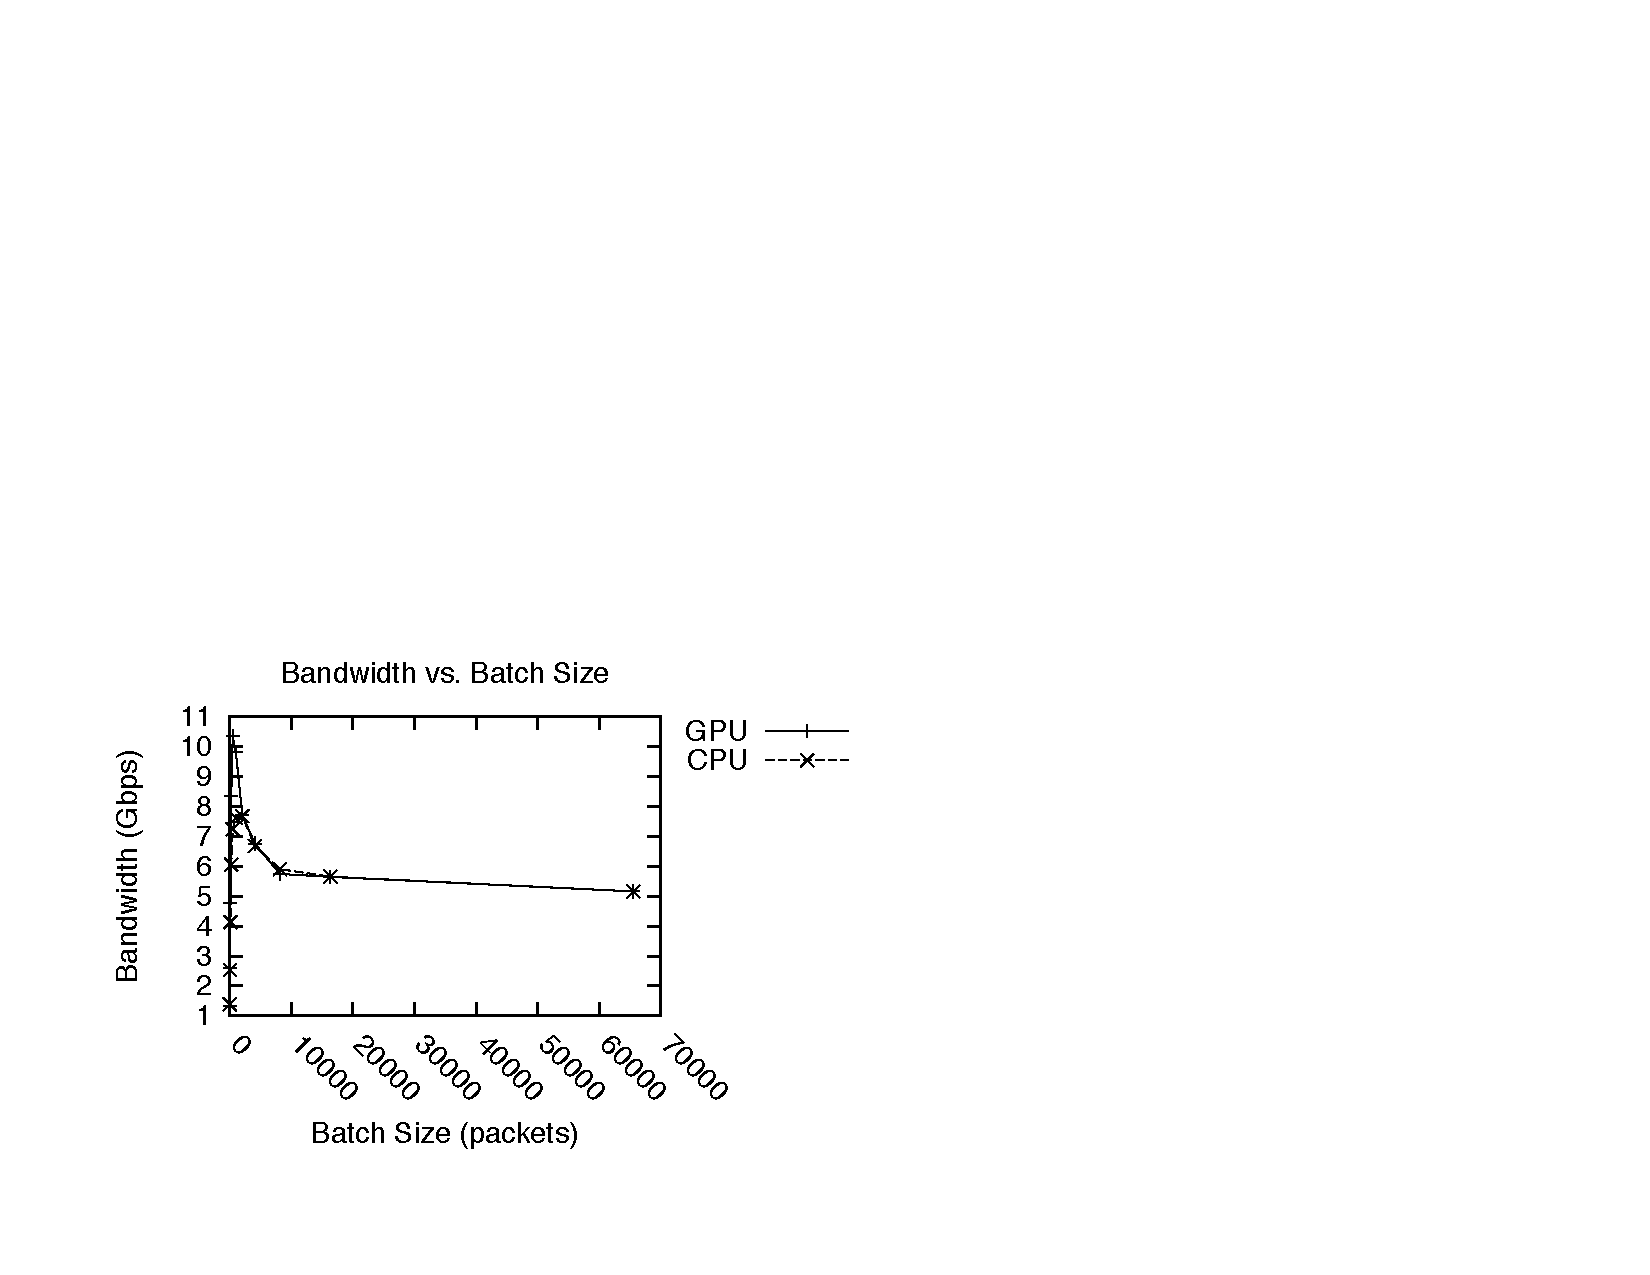
\includegraphics[height=4cm]{figs/batch_size_header_both_par_bw.pdf}\label{fig:iter2-bw}}

	\medskip
    \subfigure[Latency vs. Batch Size]{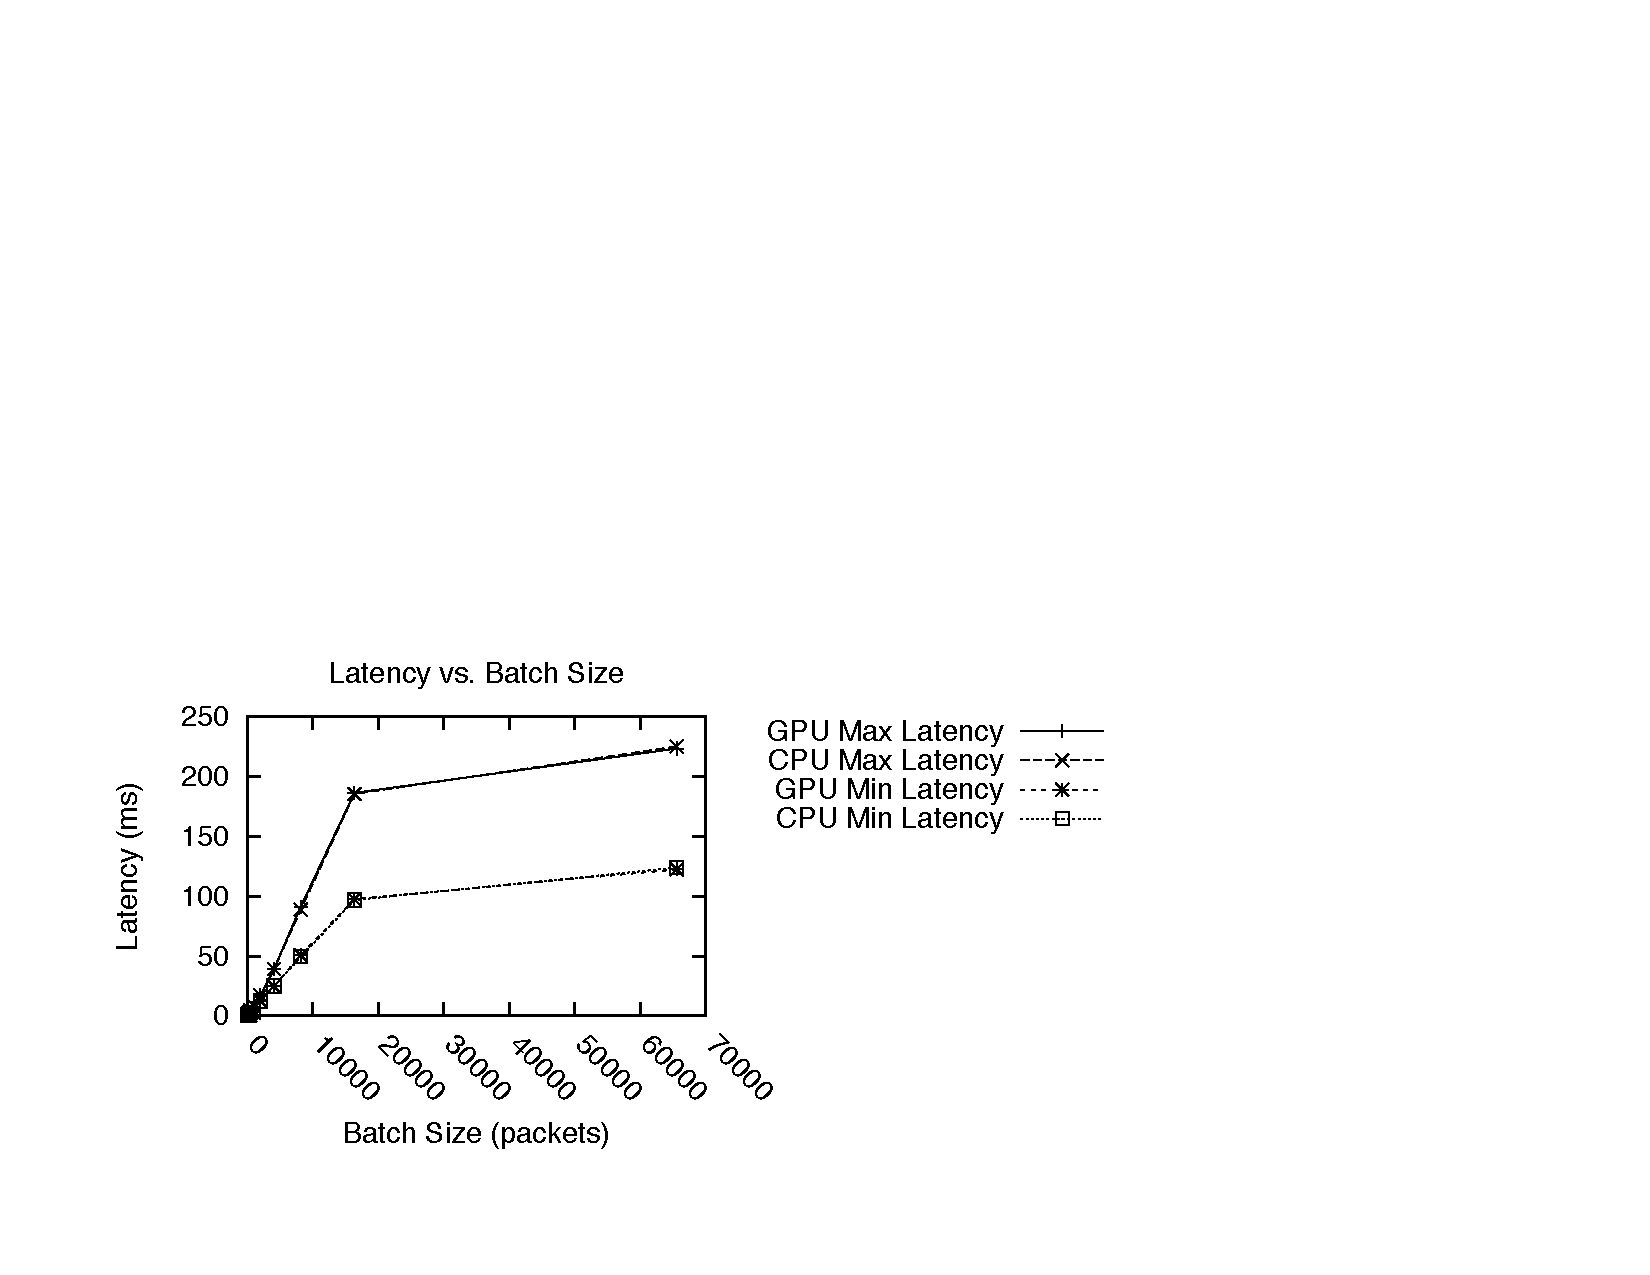
\includegraphics[height=4cm]{figs/batch_size_header_both_par_lat.pdf}\label{fig:iter2-lat}}

   	\medskip
	\subfigure[Breakdown of Relative GPU Time]{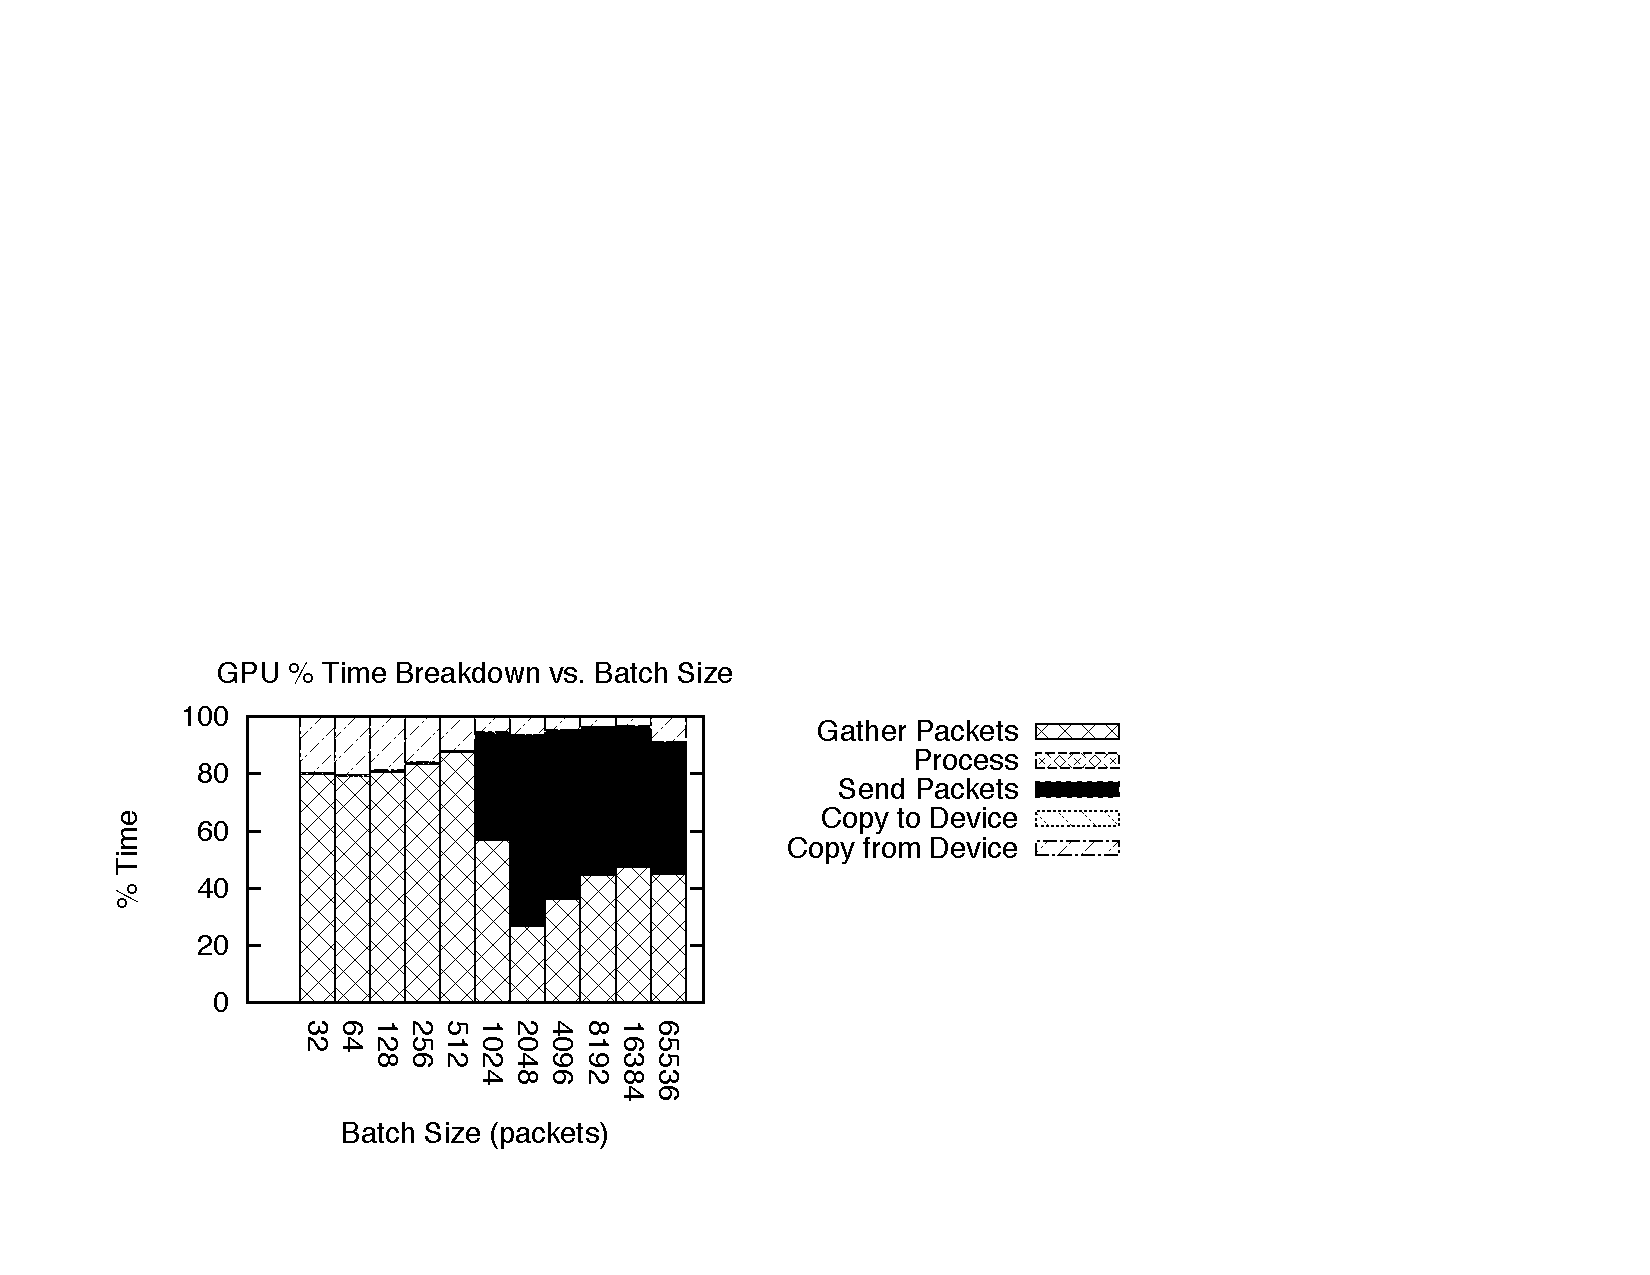
\includegraphics[height=4cm]{figs/batch_size_header_both_par_gpu_p.pdf}\label{fig:iter2-gpu-breakdown}}

    \caption{Iteration 2 Results}
	\label{fig:iter2}
\end{figure}


\subsubsection{Iteration Three}

Unfortunately, there is no unnecessary data being copied back from the GPU as
there was being copied to it; we must find another way to reduce the
copy-from-GPU overhead. Instead, we modify our router's workflow to take
advantage of mapped memory (\S\ref{sec:gpu-issues}).

This gives the CPU/GPU router a tiny edge over the CPU-only router
(Figure~\ref{fig:iter3}), but the gains are small (as Amdahl's Law would
suggest --- the copy-from-device time we eliminated was a small portion of the
total time in Figure~\ref{fig:iter2-gpu-breakdown}).


\begin{figure} e
    \centering
    \subfigure[Bandwidth vs. Batch Size]{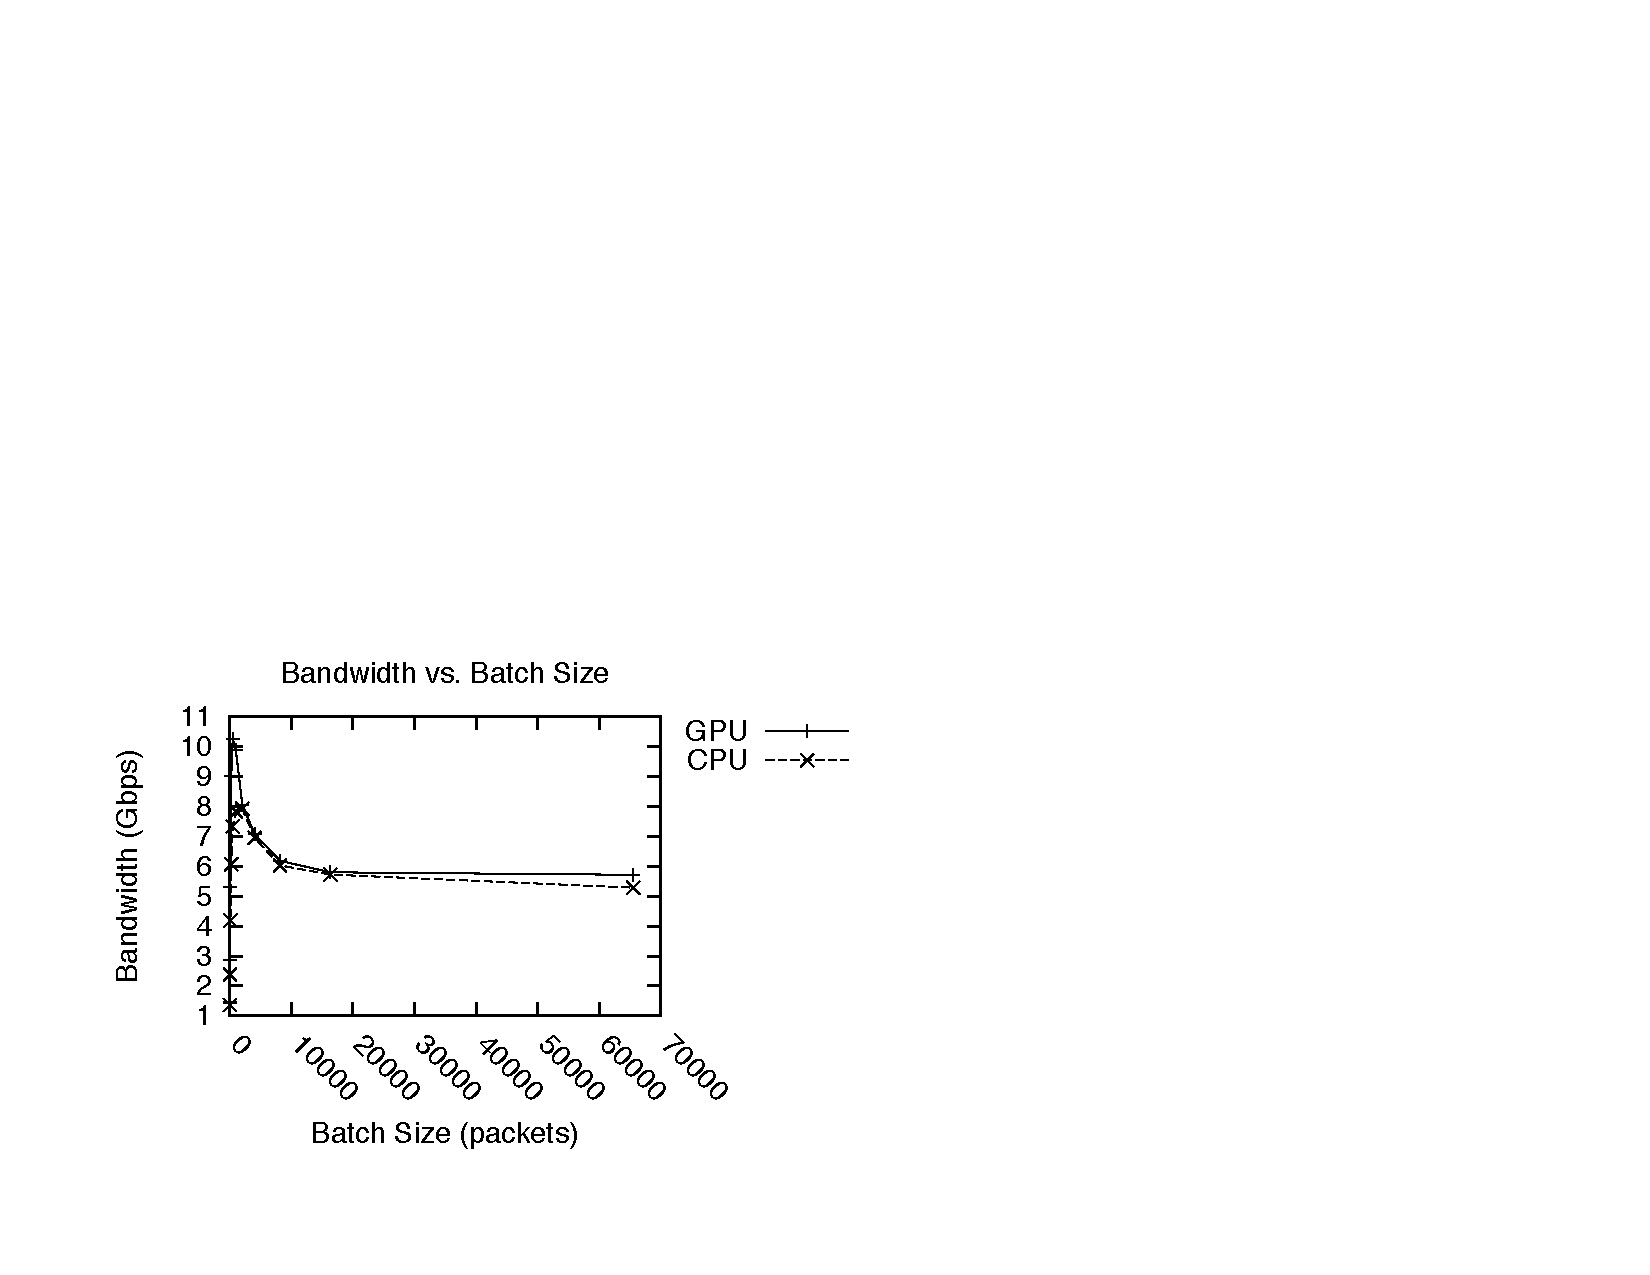
\includegraphics[height=4cm]{figs/batch_size_header_pinned_both_par_bw.pdf}\label{fig:iter3-bw}}

	\medskip
    \subfigure[Latency vs. Batch Size]{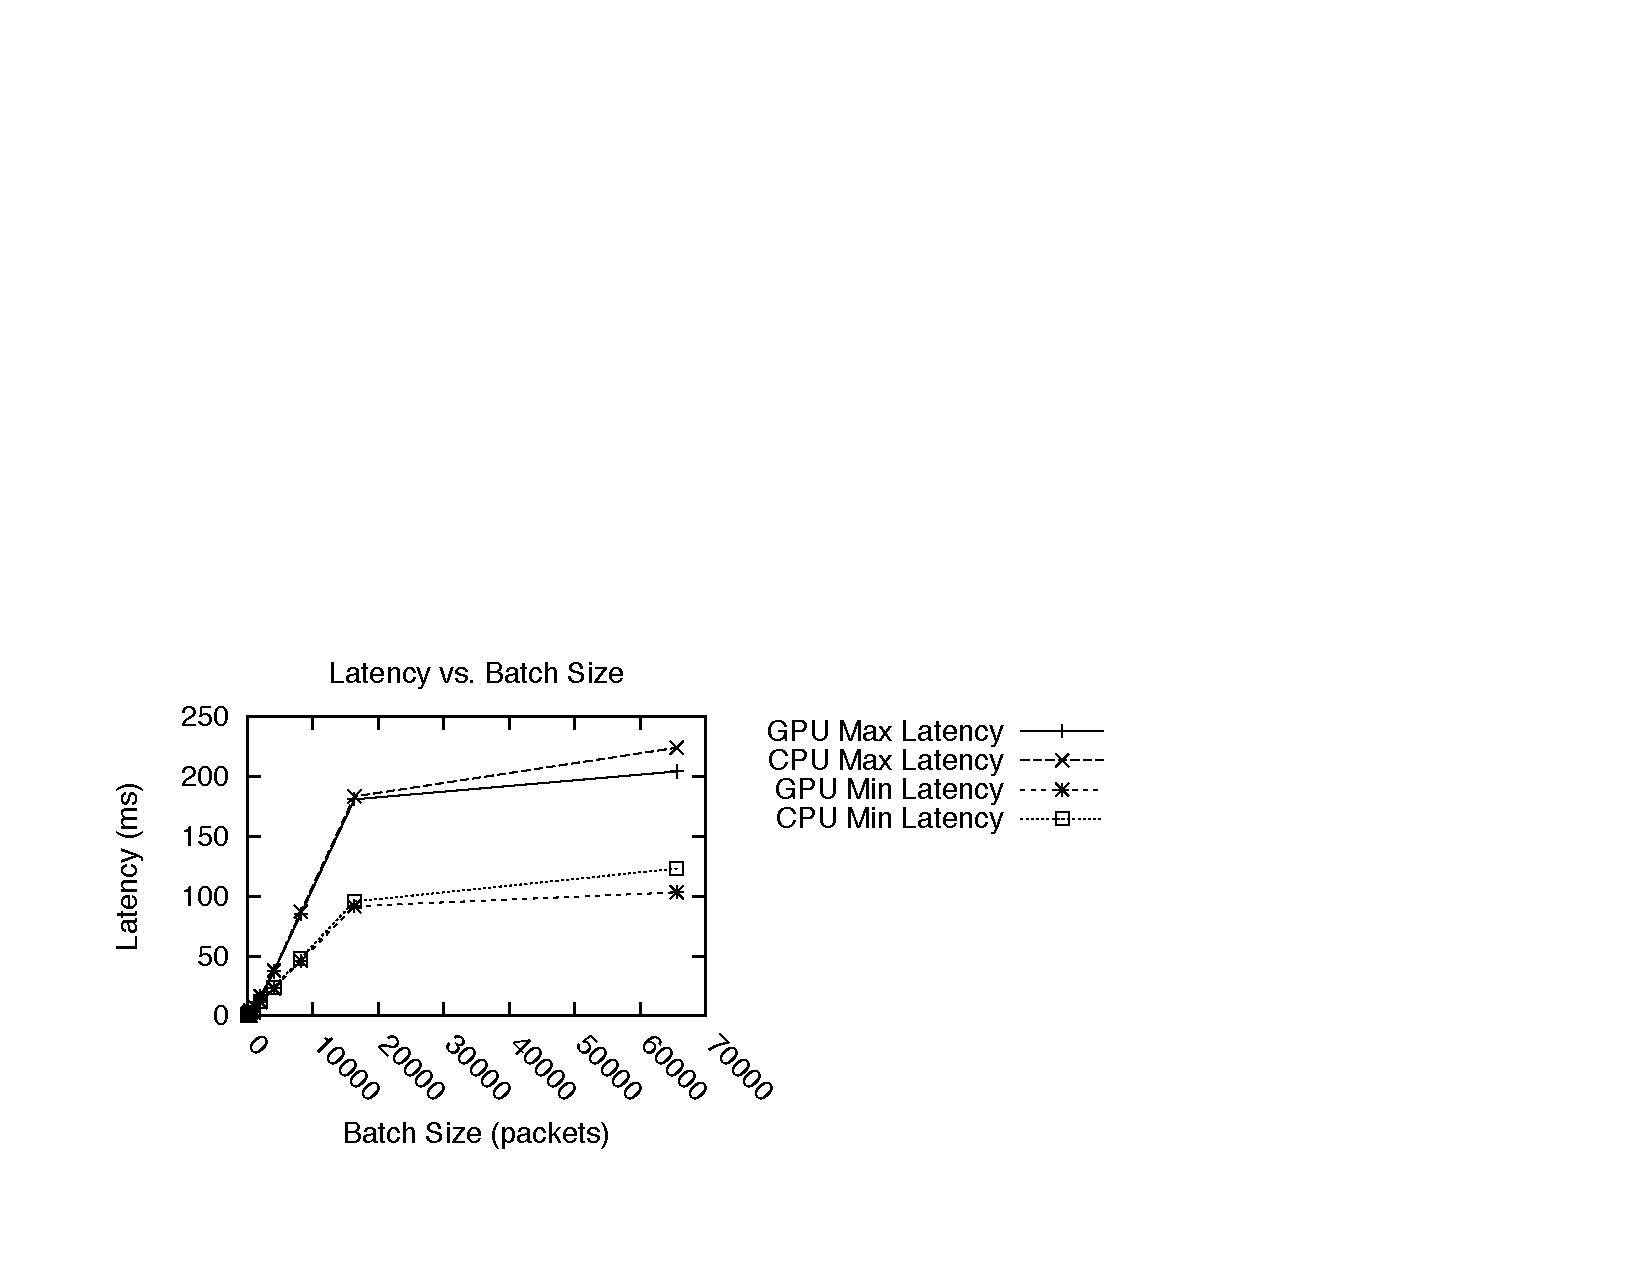
\includegraphics[height=4cm]{figs/batch_size_header_pinned_both_par_lat.pdf}\label{fig:iter3-lat}}

   	\medskip
	\subfigure[Breakdown of Relative GPU Time]{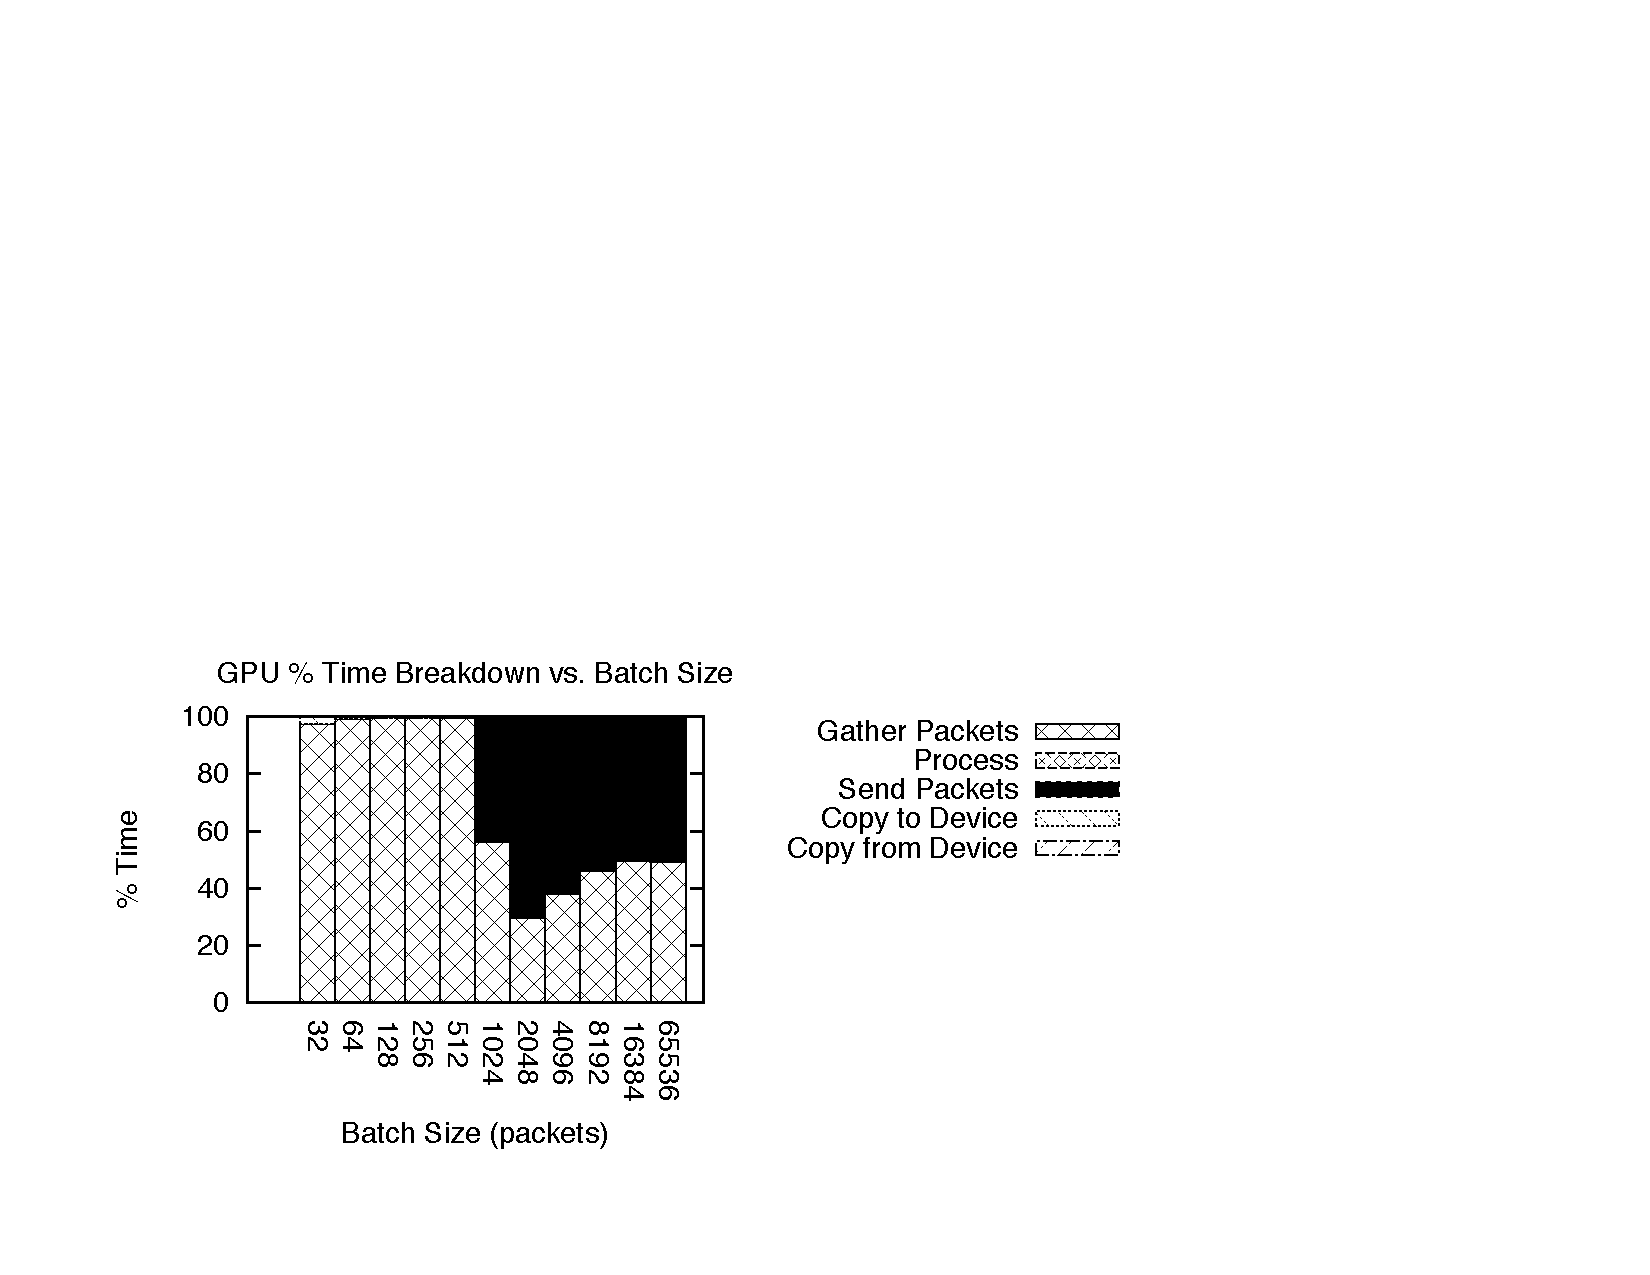
\includegraphics[height=4cm]{figs/batch_size_header_pinned_both_par_gpu_p.pdf}\label{fig:iter3-gpu-breakdown}}

    \caption{Iteration 3 Results}
	\label{fig:iter3}
\end{figure}


\subsubsection{Iteration Four}

Having eliminated the overhead of copying data to and from the GPU, the third
iteration of our CPU/GPU router only displays meager gains over the CPU-only
version. We turn to a breakdown by function of the absolute runtime of each
(Figure~\ref{fig:iter3-breakdown}) to understand why.
\begin{figure*}
    \centering
    \subfigure[Breakdown of Absolute GPU Time]{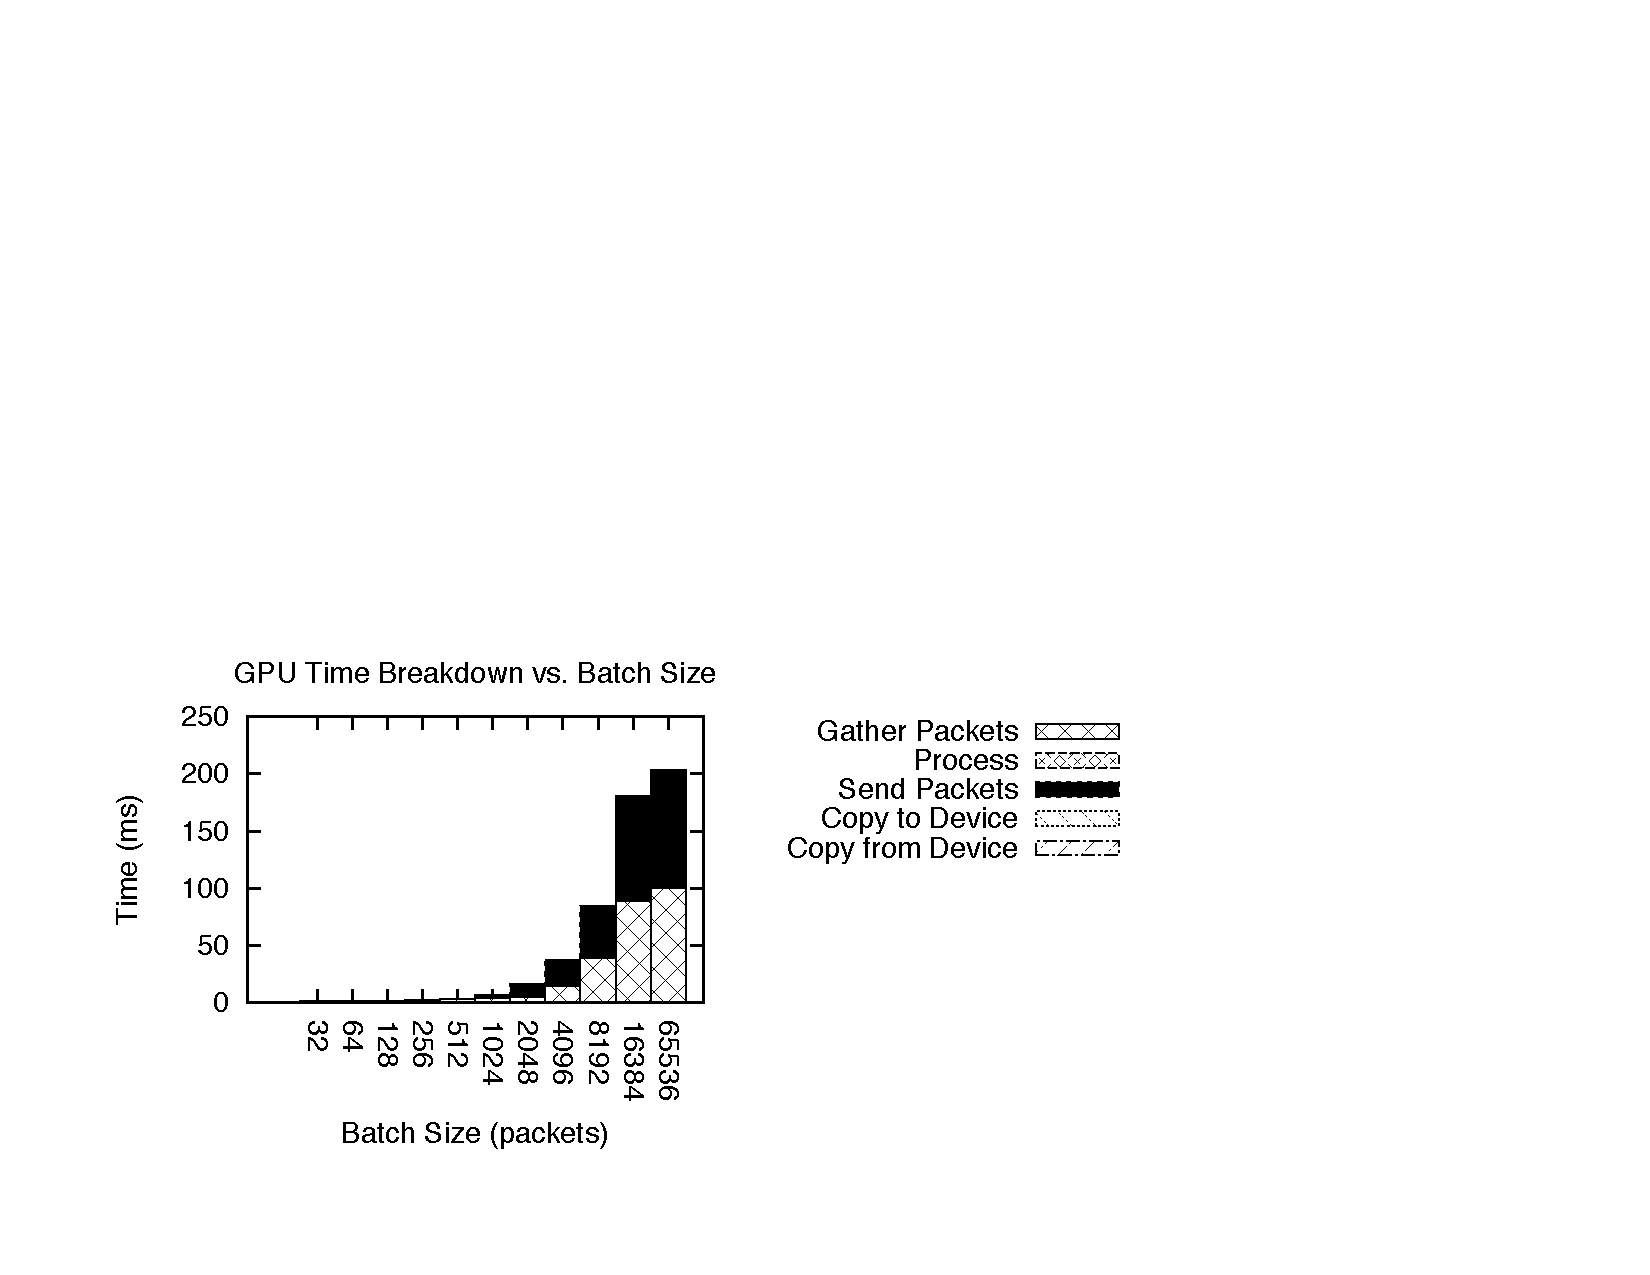
\includegraphics[height=3.7cm]{figs/batch_size_header_pinned_both_par_gpu.pdf}\label{fig:iter3-gpu-breakdown}}
	\quad
    \subfigure[Breakdown of Absolute CPU Time]{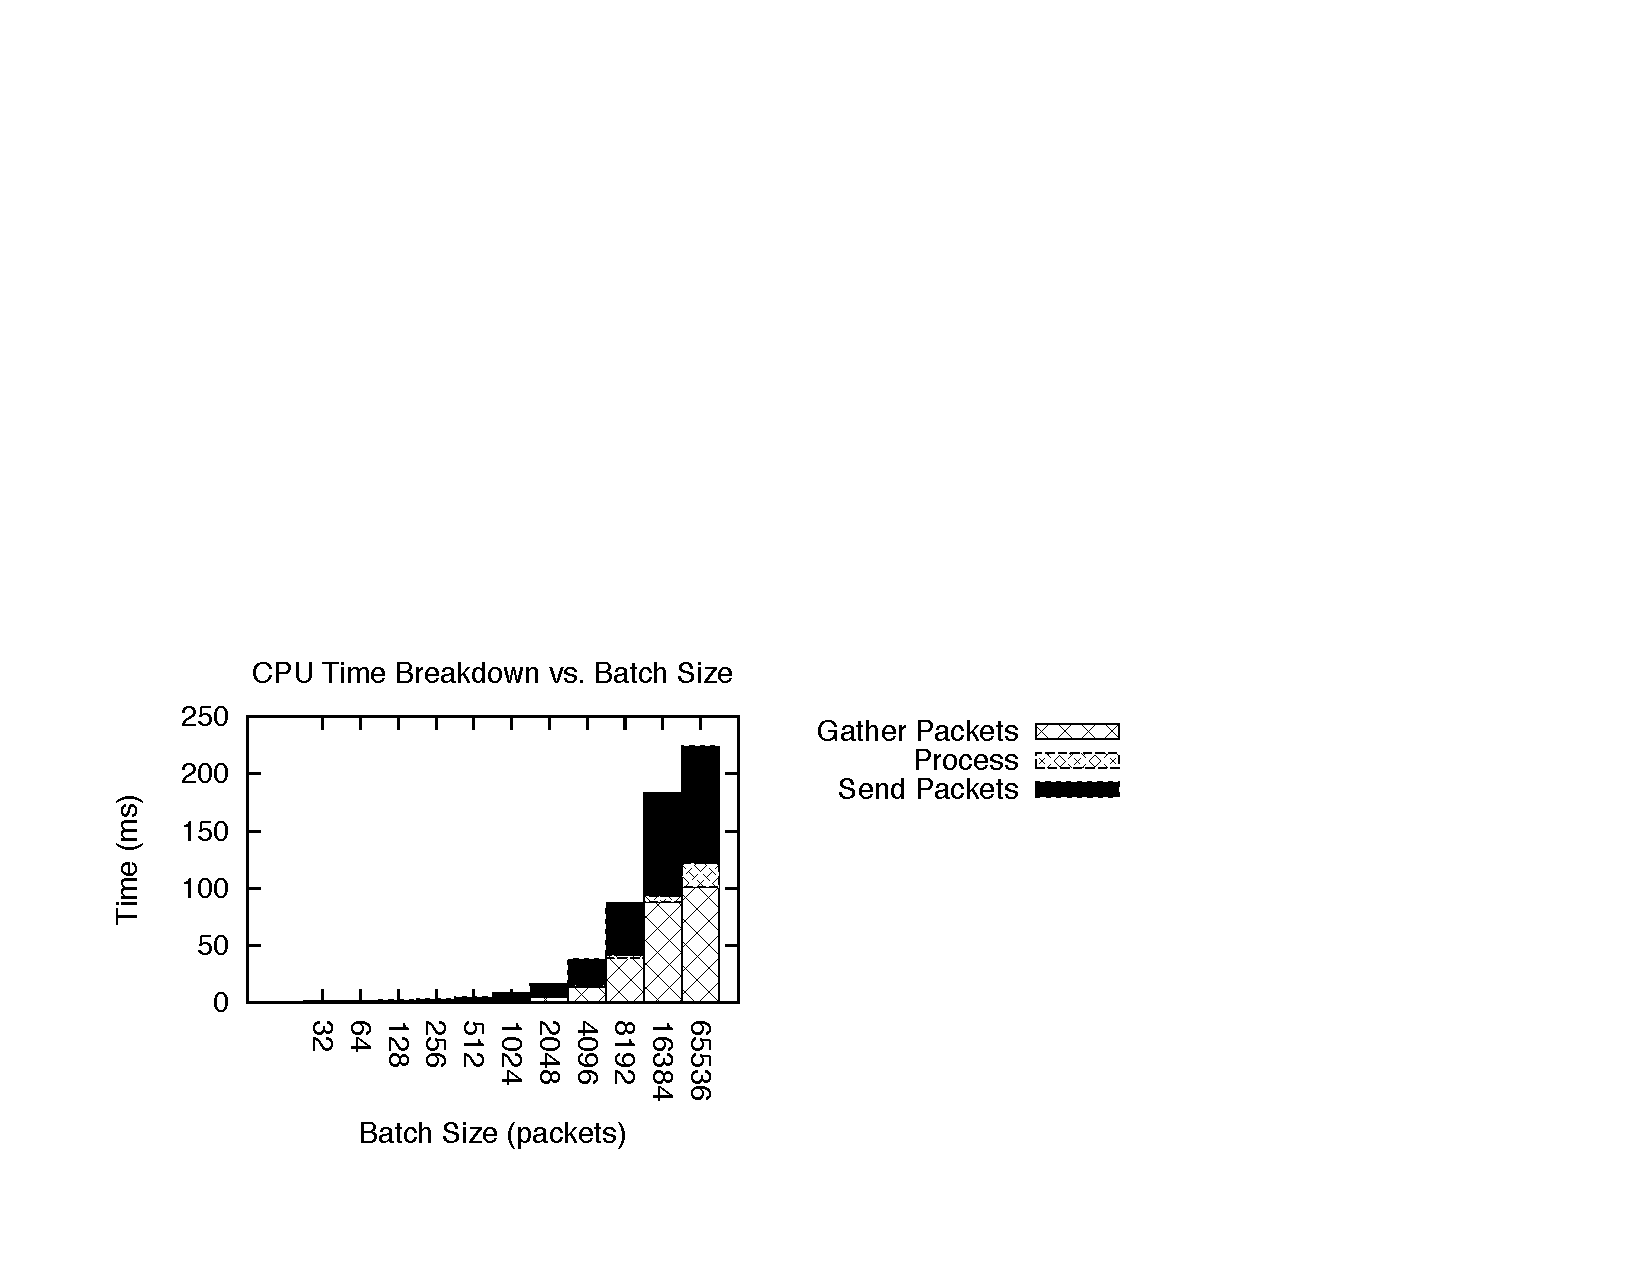
\includegraphics[height=3.7cm]{figs/batch_size_header_pinned_both_par_cpu.pdf}\label{fig:iter3-cpu-breakdown}}

    \caption{Iteration 3 Breakdown}
	\label{fig:iter3-breakdown}
\end{figure*}

The CPU-only router clearly spends more time in the processing function;
however, both spend nearly all their time performing packet I/O (that is,
receiving packets from Click and forwarding them after processing), so the
difference is processing times has little effect. This suggests that our
Click-based packet generator is the bottleneck. (Indeed, PacketShader spent a
great amount of time developing highly optimized drivers for their NIC
\cite{Han}.) To test this hypothesis, we implemented a version of our packet
generator that pre-generates a buffer of random packets and returns this buffer
immediately when queried for a new batch; similarly, when results are returned
so that packets may be forwarded, the call returns immediately rather than
waiting for the whole batch to be sent.

Sure enough, the CPU/GPU router now operates at 3X the bandwidth of the
CPU-only version and with $1/5$th the latency (Figure~\ref{fig:iter4}). Of
course, the bandwidth achieved by both is completely unrealistic (instantaneous
packet I/O is impossible), but these results indicate that with optimized
packet I/O drivers like PacketShader's, our CPU/GPU router would indeed
outperform our CPU-only one.

\begin{figure*}
    \centering
    \subfigure[Bandwidth vs. Batch Size]{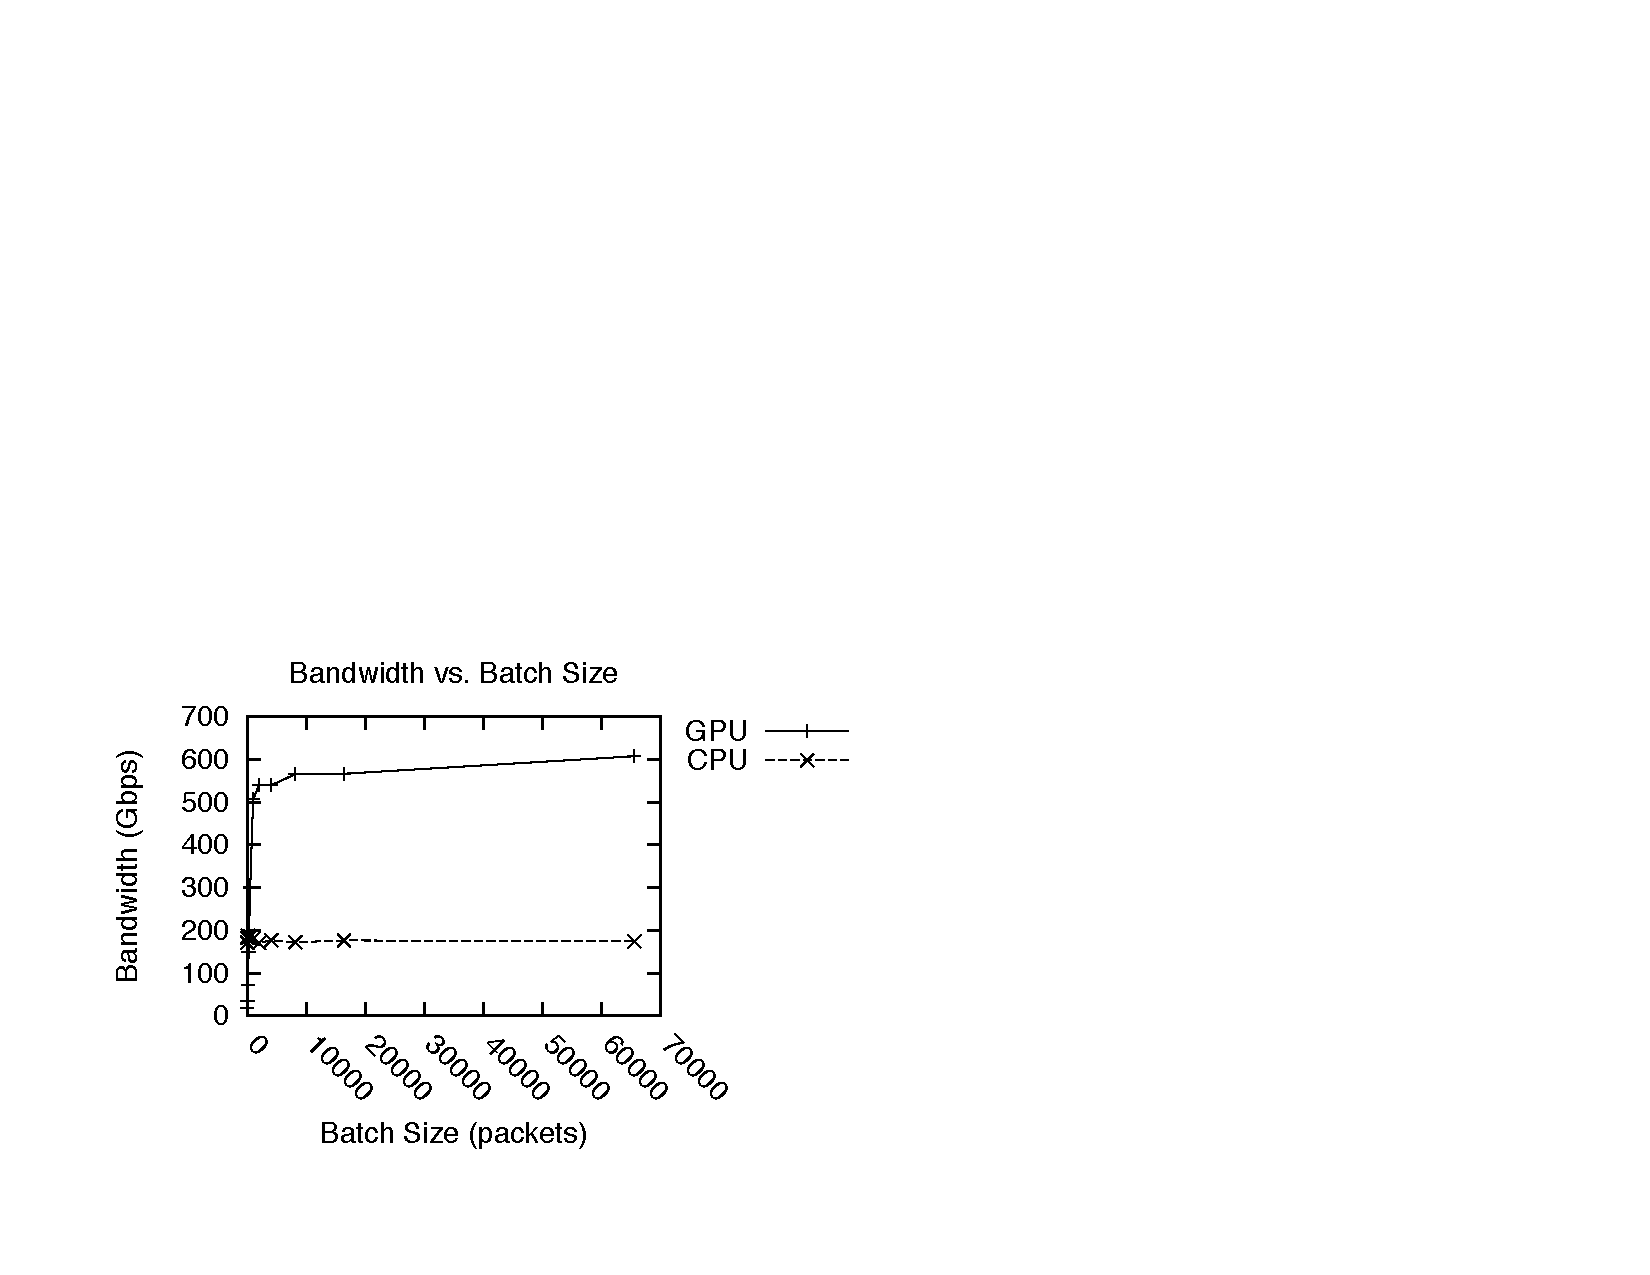
\includegraphics[height=4.5cm]{figs/batch_size_header_pinned_immediate_both_par_bw.pdf}\label{fig:iter4-bw}}
	\quad
    \subfigure[Latency vs. Batch Size]{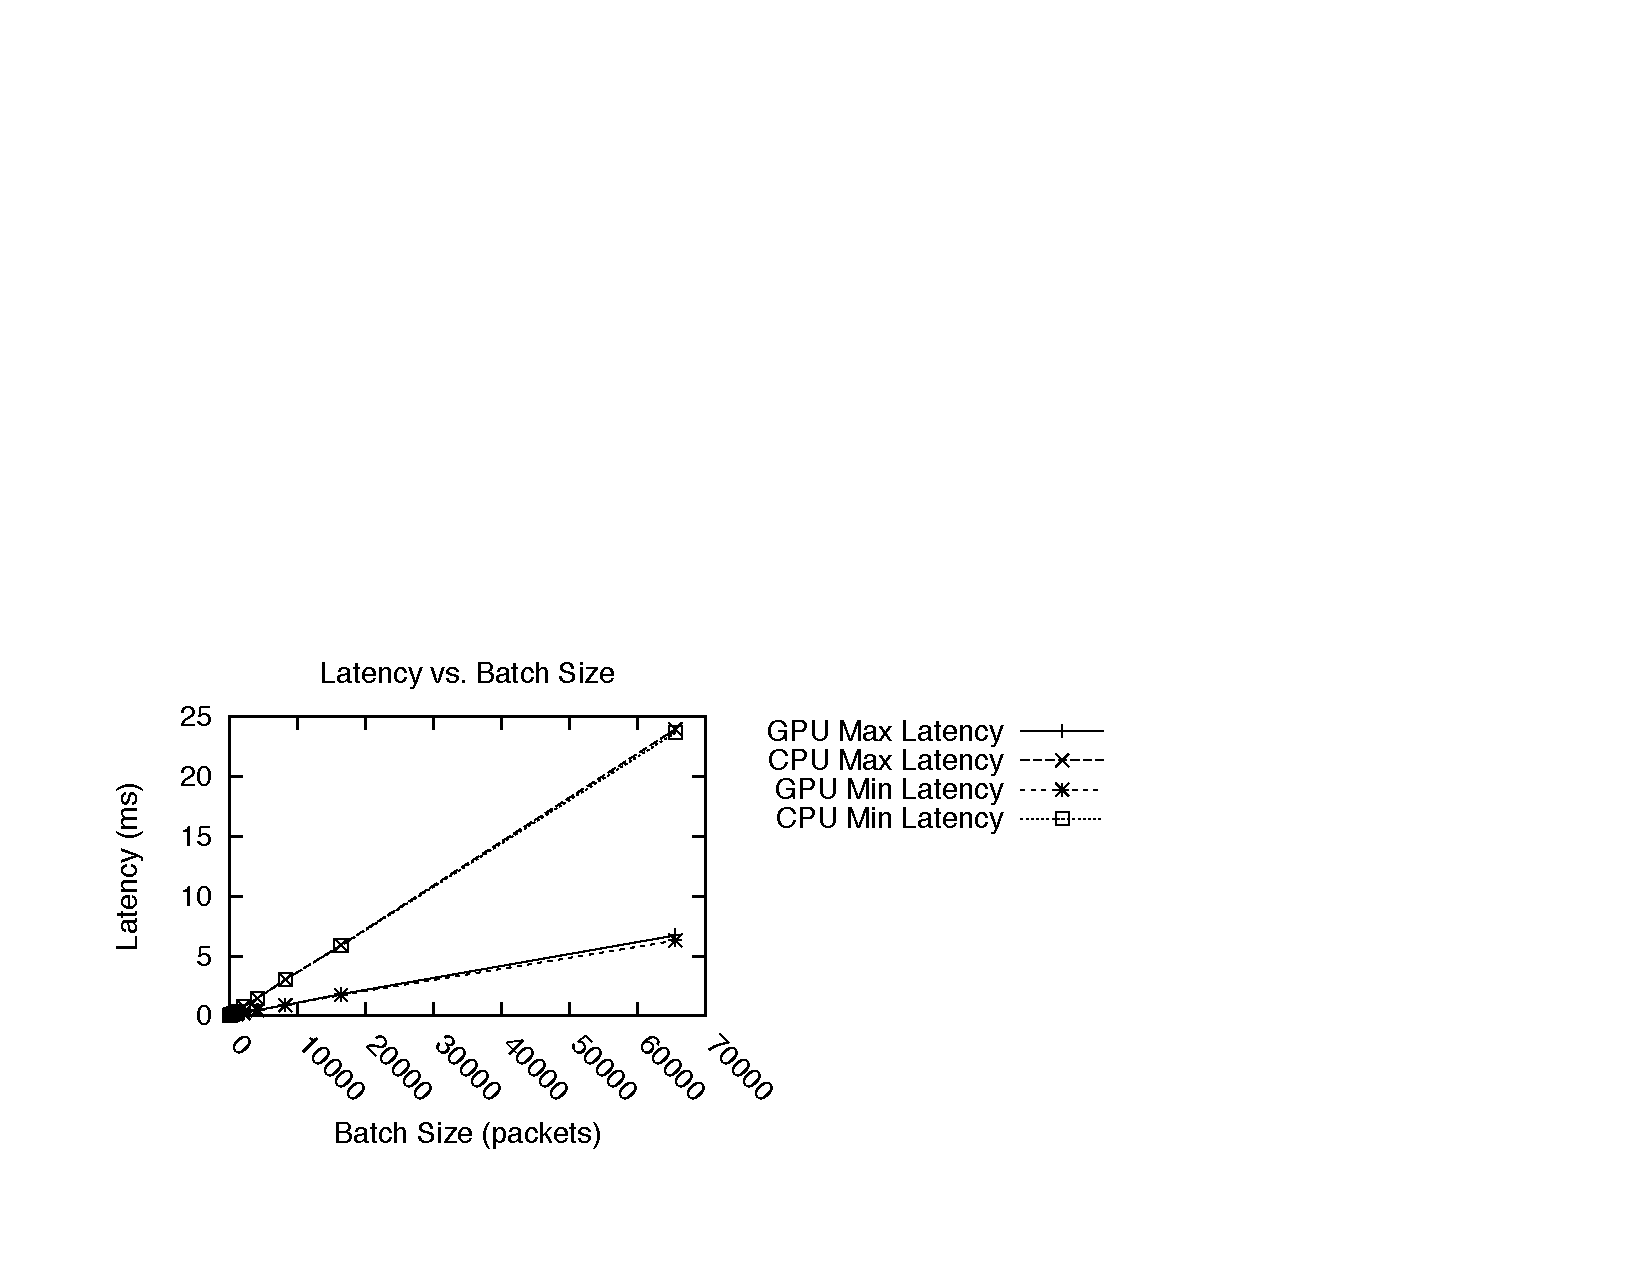
\includegraphics[height=4.5cm]{figs/batch_size_header_pinned_immediate_both_par_lat.pdf}\label{fig:iter4-lat}}

    \caption{Iteration 4 Results}
	\label{fig:iter4}
\end{figure*}
